\documentclass[11pt,letterpaper]{article}
\usepackage[margin=0.7in]{geometry}
\usepackage{fontspec}\setmainfont{Times New Roman}
\usepackage{amsmath,amssymb,booktabs,graphicx,fancyhdr}
\usepackage[hidelinks]{hyperref}
\pagestyle{fancy}\fancyhf{}\lhead{Return screening: methods and results}\rhead{19 November 2026}\cfoot{\thepage}
\setlength{\headheight}{14pt}\renewcommand{\headrulewidth}{0.3pt}
\setlength{\parindent}{0pt}\setlength{\parskip}{5pt}
\setlength{\abovedisplayskip}{5pt}\setlength{\belowdisplayskip}{5pt}
\setlength{\tabcolsep}{7pt}\renewcommand{\arraystretch}{1.06}
\newcommand{\subhead}[1]{\vspace{3pt}{\large\bfseries #1}\par}
\newcommand{\ind}{\mathbf 1}
\begin{document}
\begin{center}{\LARGE\bfseries Return screening: methods and results}\end{center}

Phelim, I have compared which checks earn their place when we allow a fixed amount of follow-up work. The useful question is whether different checks cover different reporting problems, and whether adding a third or fourth check improves coverage.

\subhead{Data and the starting point}
The main sample is 194 Chen--Zimmermann long--short stock portfolios. I use 1980--2004 to develop the score scales, 2005--2016 to set cutoffs and choose combinations, and January 2017--December 2025 to evaluate them ($T=108$ months). These are published gross excess payoffs, not fund NAVs; the risk-free return is not subtracted again.

The first exercise found one conventional warning among 195 complete histories. In the 194-name core, raising the cutoff on the same score reduced three-month delayed-loss warnings from 111 to 66, while unchanged warnings fell from one to zero. That fixed-1\% loss experiment shows the cost of a tighter warning threshold. The new comparison also changes the checks themselves.

\subhead{What each check measures}
For each complete, nonconstant record $x_1,\ldots,x_T$, calculate its mean $\bar x$, sample standard deviation $s>0$ and mean/SD ratio $h=\bar x/s$. The four scores are:
\[
 B=\frac{\#\{0\leq x_t\leq s\}}{1+\#\{-s\leq x_t<0\}},\qquad
 D=T\Phi(-h)-\#\{x_t<0\},\qquad
 A=\frac{\sum_{t=2}^{T}(x_t-\bar x)(x_{t-1}-\bar x)}{\sum_{t=1}^{T}(x_t-\bar x)^2}.
\]
$B$ compares small gains with small losses. $D$ measures the shortage of losses relative to a fitted normal distribution ($\Phi$ is its standard CDF). $A$ measures signed lag-one dependence. For local bunching, put $b=s/4$ and count observations in four bins:
\[
 L_2:[-2b,-b),\quad L_1:[-b,0),\quad G_1:(0,b],\quad G_2:(b,2b],\qquad
 Z=\frac{3(G_1-L_1)-(G_2-L_2)}{\sqrt{9(G_1+L_1)+G_2+L_2}}.
\]
Set $Z=0$ if the denominator is zero. Exact zeros enter $B$'s numerator but no $Z$ bin. The contrast cancels the expected contribution of a locally linear density slope. All four scores warn in their upper tails using historical cutoffs. $Z$ is empirically calibrated; $D$ is the paper's Gaussian loss-count adaptation.

\subhead{How I combine them}
Development supplies $M_{\rm dev}=3{,}148$ complete, overlapping, December-ending 108-month records. Score $S_j(x)$ becomes a historical rank
\[
 u_j(x)=\frac{\#\{k:S_{kj}\leq S_j(x)\}}{M_{\rm dev}+1}.
\]
For any subset $J$, order its ranks $u_{(1)}\geq\cdots\geq u_{(|J|)}$ and use
\[
 C_J^{\rm OR}=\max_{j\in J}u_j,\qquad
 C_J^{\rm maj}=u_{(\lfloor |J|/2\rfloor+1)},\qquad
 C_J^{\rm mean}=|J|^{-1}\sum_{j\in J}u_j.
\]
OR and strict majority give 26 distinct arrangements, counting each singleton once. Eleven nonsingleton mean-rank combinations and one principal-component comparator give 38. The latter is $C^{\rm PC}=w^\top((u_j-\mu_j)/\sigma_j)_{j=1}^4$: calibration data set the means, standard deviations and leading covariance eigenvector $w$, oriented to have nonnegative component sum (a tie makes its largest absolute component positive).

\newpage
\subhead{The reporting changes}
I apply known changes to observed histories so we can measure what each screen notices. Let $s_0$ be the original record's standard deviation. Eligible losses satisfy $I_t=\ind\{-0.25s_0\leq x_t<0\}$ and are initially replaced by $g=0.0125s_0$:
\[
 q_t=[v(g)-v(x_t)]I_t,\qquad v(y_t)=v(x_t)+q_t-q_{t-L},\qquad
 v(x)=\begin{cases}x,&\text{long--short payoff},\\\log(1+x),&\text{funded NAV return}.\end{cases}
\]
I use recognition delays $L=1,3,6$ months; permanent concealment omits $q_{t-L}$. Eligibility uses the original loss, so incoming repayments cannot be hidden again. Six actual preceding months initialise the ledger, and opening/closing balances reconcile it. The funded sensitivity uses $x_t=r_{f,t}+LS_t>-1$, with long and short books each equal to equity. A separate smoothing change is
\[
 y_t=(1-\lambda)x_t+\lambda x_{t-1},\qquad \lambda\in\{0.25,0.50,0.75\}.
\]
Each altered record gets its own recomputed diagnostic mean and standard deviation. The reporting bound and positive target retain the original $s_0$.

\subhead{A common allowance and choices made on older data}
I resample the 2005--2016 calibration panel jointly in circular 12-month calendar blocks: 5,000 draws, each containing 194 histories. This keeps cross-strategy dependence. For sorted calibration scores $c_{(1)}\leq\cdots\leq c_{(M)}$, each full rule $r$ gets
\[
 \tau_{r,\alpha}=c_{(\lceil(1-\alpha)M\rceil)},\qquad
 \text{warn when }C_r(x)>\tau_{r,\alpha}.
\]
The grid is $\alpha=0,0.01,\ldots,1$; endpoints use $+\infty,-\infty$. Ties stay together, so realised calibration warnings may fall below the allowance.

Four hundred additional old-data resamples choose the best arrangement overall and within each number of checks. I give equal weight to permanent concealment, three-month delay and half-weight smoothing. With $N_{\rm tr}$ training records and altered version $y_i^m$, maximise new warnings:
\[
 \widehat G_r=\frac1{3N_{\rm tr}}\sum_{m=1}^3\sum_{i=1}^{N_{\rm tr}}
 \ind\{C_r(y_i^m)>\tau_{r,\alpha},\ C_r(x_i)\leq\tau_{r,\alpha}\}.
\]
Ties prefer fewer checks, then the rule ID. Equal weights specify the experiment; they do not estimate how often each reporting problem occurs.

\subhead{Reading the frontier and checking transfer}
In later data, the horizontal coordinate is the share of unchanged records warned; the vertical coordinate is the share of altered records warned:
\[
 \widehat W_r=\frac1N\sum_i\ind\{C_r(x_i)>\tau_{r,\alpha}\},\qquad
 \widehat H_{r,m}=\frac1N\sum_i\ind\{C_r(y_i^m)>\tau_{r,\alpha}\}.
\]
The graphs hold the older-data 5\% choice for each check count fixed and vary its cutoff; $B+D$ is the prespecified comparator. This separates choosing checks from choosing the warning threshold. A best-looking later-data envelope would describe this sample, rather than a choice made beforehand.

Transfer checks use five folds holding whole economic strategy categories out of all fitting (1,000 calibration and 200 selection draws), and 500 paired joint-calendar resamples with choices fixed. Sensitivities cover 60-month histories, six-month blocks, wider local bins, fixed 1\% loss bounds, half-application and historical-winner weighting. The earlier exercise had already examined the 2017--2025 sample. The workbook gives the full results and source definitions.

\newpage
\subhead{What we learn}
For the 194 US histories, higher means more changes noticed; further right means more follow-up work. Dots mark the 5\% older-reference allowance. Both graphs show the 0--12\% realised-warning region.
\begin{center}
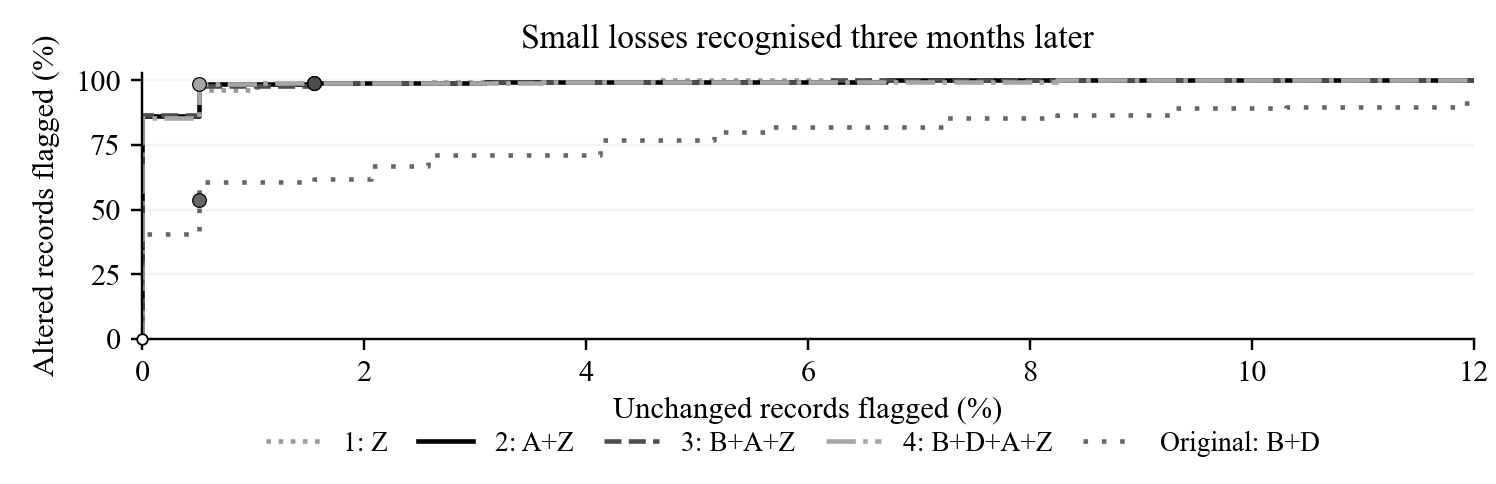
\includegraphics[width=0.98\linewidth]{figures/report_loss_delay.png}\\[-2pt]
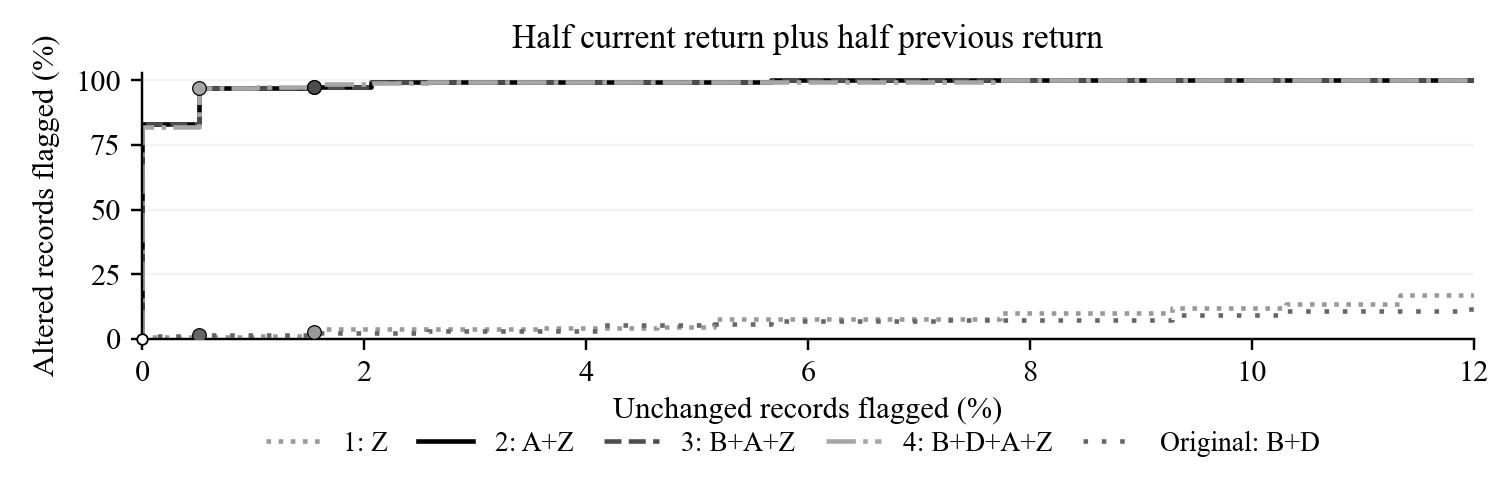
\includegraphics[width=0.98\linewidth]{figures/report_smoothing.png}
\end{center}
At that 5\% allowance, total warning counts are (World: Jensen--Kelly--Pedersen factors):
\begin{center}
\begin{tabular}{llrrr}\toprule
Data & Record & $N$ & Original $B+D$ & Local/serial $A+Z$\\\midrule
US & Unchanged & 194 & 1 & 3 \\
US & Three-month delay & 194 & 104 & 192 \\
US & Half-weight smoothing & 194 & 3 & 189 \\
\midrule
World & Unchanged & 153 & 6 & 3 \\
World & Three-month delay & 153 & 79 & 152 \\
World & Half-weight smoothing & 153 & 5 & 153 \\
\bottomrule\end{tabular}
\end{center}
Local bunching and serial dependence cover different changes. Two- and three-check choices perform almost identically here; a fourth does not consistently improve coverage. In world factors, $A+Z$ catches more changes with fewer unchanged warnings.

Chen--Pelger--Zhu's gross model portfolio has monthly excess Sharpe 1.53 in 1992--2000; our screening reference ends in 1991. At the 5\% allowance, all 38 rules are initially quiet. After four small losses are deferred three months, $A+Z$ stays quiet, while $B+A+Z$ and $B+D$ flag. That supports complementary coverage, rather than one ideal check count.

I would develop that operating lesson. \href{https://doi.org/10.1093/rfs/hhs085}{Bollen--Pool (2012)} already combines flags, and \href{https://doi.org/10.2308/TAR-2020-0068}{Beneish--Vorst (2022)} studies investigation costs. The frontier is established; our possible contribution is evidence about where fixed choices transfer or fail. These experiments measure detection of imposed changes, not verified fraud.
\end{document}
